\documentclass[11pt]{article}

% parameters are fairly self-explanatory here, thankfully
\usepackage[width=7in,height=9.5in,top=0.75in,centering]{geometry}

% for math-ing
\usepackage{amsmath}
\usepackage{amssymb}


%%%%%% tables %%%%%%%%

\usepackage{array}
\renewcommand{\arraystretch}{1.5}
\setlength{\tabcolsep}{8pt}

%%%%%% plotting %%%%%%

\usepackage[dvipsnames]{xcolor}
\usepackage{tikz}
\usepackage{pgfplots}

\pgfplotsset{every axis/.append style={
                    axis x line=middle,    % put the x axis in the middle
                    axis y line=middle,    % put the y axis in the middle
                    axis line style={<->,color=black}, % arrows on the axis
                    xlabel={$x$},          % default put x on x-axis
                    ylabel={$y$},          % default put y on y-axis
            }}
            
 \pgfplotsset{compat=1.14} % sometimes, everything falls apart without this
 
 %\usepgfplotslibrary{fillbetween} %for shading between curves

%%%%%% commands %%%%%%

% exam heading; course name is first argument, exam information is second argument
\newcommand{\Heading}[2]{
    \fbox{
        {\Large\textbf{#1}}
        }
    \hfill
    \fbox{
        \begin{minipage}{0.2\textwidth}
            \begin{center}
            \textbf{#2}
            \end{center}
        \end{minipage}
    }
    \par\vspace{0.1in}}

% for being lazy while beautifying integrals
\newcommand{\dint}{\displaystyle\int}

% for being lazy while beautifying limits
\newcommand{\dlim}{\displaystyle\lim}

%%%%%% stuff %%%%%%

\usepackage{fancyhdr}

%\setcounter{page}{0} % first page is page 0

\parindent0pt % no indent

\fboxsep=0.25cm % little space in fbox border

%%%%%% BEGIN! %%%%%%%

\begin{document}

\pagestyle{fancy}

% record goals here to create sense of transparency

\fancyhead[c]{%
  \ifcase\value{page}
  % empty test for page = 0
  \or {}% 
  \or
  \or {\bf\color{ForestGreen} FE1(D1): Meaning of a Derivative}% page=1
  \or {\bf\color{ForestGreen} FE2(D3): Derivatives of Basic Functions}% page = 2
  \or {\bf\color{ForestGreen} FE3(D2): Compute Derivatives}% page = 3
  \or {\bf\color{Fuchsia} FE4(I1): Meaning of an Integral}% page = 4
  \or {\bf\color{Fuchsia} FE5(I3): Antiderivatives and Indefinite Integrals}% page = 5
  \or {\bf\color{Fuchsia} FE6(I4): Compute Definite Integrals}% page = 6
  \or {\bf\color{ProcessBlue} FE7(F3): Summations}% page = 7
  \or {\bf\color{RoyalBlue} FE8(L1): Limits and Continuity}% page = 8
  \or {\bf\color{Orange} FE9(P1): Discrete Random Variables}
  \or {\bf\color{Orange} FE10(P2): Continuous Random Variables}
  \else
  % Empty chead here!
  \fi
}

\thispagestyle{empty} % don't display that this is page 0

\Heading{MATH 1190/1210 Survey of Calculus I}{Final Exam\\Solutions\\Fall 2025}

\vspace{0.1in}

\textbf{Name} \hrulefill \, \begin{minipage}{0.16\textwidth}\begin{center}\textbf{UVA ID\\ (e.g. hdj4nd)} \end{center}\end{minipage}\hrulefill\\

\begin{minipage}{0.2\textwidth}\begin{center}\textbf{Course \&\\ Section Number} \end{center}\end{minipage} \hrulefill\,\,\textbf{Date} \hrulefill  \\

\hrulefill
\paragraph*{Course \& Section Numbers:}

{\small
\begin{center}
\begin{tabular}{| c | c | c | c | c |}
\hline
%
\begin{minipage}{0.12\textwidth}\begin{center}
1190-100\\
J. Rolf\\
(11:00 AM)
\end{center}\end{minipage}
&
\begin{minipage}{0.12\textwidth}\begin{center}
1190-200\\
J. Rolf\\
(9:30 AM)
\end{center}\end{minipage}
&
\begin{minipage}{0.12\textwidth}\begin{center}
1210-100\\
Mikhail\\
(8 AM)
\end{center}\end{minipage}
&
\begin{minipage}{0.12\textwidth}\begin{center}
1210-200\\
Raul\\
(9:30 AM)
\end{center}\end{minipage}
&
\begin{minipage}{0.12\textwidth}\begin{center}
1210-300\\
Sherman\\
(11 AM)
\end{center}\end{minipage}
\\
%
\hline
%
\begin{minipage}{0.12\textwidth}\begin{center}
1210-400\\
Sherman\\
(12:30 PM)
\end{center}\end{minipage}
&
\begin{minipage}{0.12\textwidth}\begin{center}
1210-500\\
Michael\\
(2 PM)
\end{center}\end{minipage}
&
\begin{minipage}{0.12\textwidth}\begin{center}
1210-600\\
J. Bowling\\
(3:30 PM)
\end{center}\end{minipage}
&
\begin{minipage}{0.12\textwidth}\begin{center}
1210-700\\
Josh\\
(9:30 AM)
\end{center}\end{minipage}
&
\begin{minipage}{0.12\textwidth}\begin{center}
1210-800\\
Mason\\
(2 PM)
\end{center}\end{minipage}
\\
%
\hline
%
\begin{minipage}{0.12\textwidth}\begin{center}
1210-900\\
Caelan\\
(3:30 PM)
\end{center}\end{minipage}
&
\begin{minipage}{0.12\textwidth}\begin{center}
1210-920\\
Caelan\\
(5 PM)
\end{center}\end{minipage}
&
\begin{minipage}{0.12\textwidth}\begin{center}
1210-940\\
Mitchell\\
(10 AM)
\end{center}\end{minipage}
&
\begin{minipage}{0.12\textwidth}\begin{center}
1210-950\\
Mitchell\\
(11 AM)
\end{center}\end{minipage}
&
\begin{minipage}{0.12\textwidth}\begin{center}
1210-960\\
Mitchell\\
(noon)
\end{center}\end{minipage}
\\
\hline
\end{tabular}
\end{center}

}

{\small

\paragraph*{Instructions:}

\begin{itemize}
    
    \item The regular time allowed for completing this assessment is \fbox{$100$} minutes.
    %\item This assessment is out of 50 points.\\ 
    \item This assessment contains one single-part or multi-part problem for each of the following targets: \textbf{FE1(D1), FE2(D2), FE3(D3), FE4(I1), FE5(I3), FE6(I4), FE7(F3), FE8(L1), FE9(P1), FE10(P2)}.
    \item On each problem, you will receive a score of Exceeds Expectations (5), Proficient (4), Almost (3), Developing (2), Emerging (1), or Not Yet (0). %{\bf Please do not interpret your score as a percentage.}
    \item \textbf{It is to your best interest to complete all problems on this exam and not leave anything black.} The Final Exam learning targets count separately. If a problem is skipped, you will earn a Not Yet (0) on the corresponding Final Exam learning target, which could impact your final negatively and significantly.
    \item Your performance on each of the Final Exam targets can replace your scores on corresponding targets from Knowledge Checkpoints given during the semester, if your performance on the Final Exam is higher.
    %\item You will have opportunities to reassess on the targets appearing on this assessment after the next {\bf 2} assessments.\\
    \item You may NOT use calculators, dictionaries, notes, phones, or any other kind of aid.
    \item Please write neatly. What cannot be read, cannot be graded.
    \item Carefully work out each problem and clearly indicate your final answer to every problem.
    \item Throughout, give the most descriptive answer possible. \textbf{For instance, ``DNE" will not be accepted when ``$=\infty$" is applicable.}
    %\item Please provide the most specific answer possible. For instance, if a limit does not exist because it goes to $\infty$ or $-\infty$, then specify this.
    \item Please use the methods discussed up to this point in the course. For example, any work based on l'H\^opital's Rule will not receive credit.
    \item \textbf{All work must be shown unless otherwise specified.} Partial credit will not be given if appropriate work is not shown.
    \item In particular, {\bf any answer appearing with no justification will receive no credit regardless of whether the answer was correct}, unless otherwise specified.
    \item Please first respond to the prompts on which you feel most proficient, then respond to others later.
    \item This booklet is printed double-sided. It contains 14 pages and 10 numbered problems.
    \end{itemize}
    
    }

\vfill


%%%%%%%%%
\newpage

This page is left blank intentionally.\\

Use this page if you need additional space to write your solutions to any problem. \\

If you wish this page graded, you must refer to this page on \textbf{the original page} of the problem. Otherwise, your grader will NOT consider your work on this page.

\newpage%
%%%%%%%%%


\begin{enumerate}

%%%%%%%%%%%%%%%%%%%%%%%%%%%%%%%%%%%%%%%%%%%%%%%%%%%%%
%%%%%%%%%%% BEGIN PROBLEM D1 %%%%%%%%%%%%%%%%%%%%%%%%
%%%%%%%%%%%%%%%%%%%%%%%%%%%%%%%%%%%%%%%%%%%%%%%%%%%%%

\item 

\begin{enumerate}
    \item The function $C(r)$ is the total cost, in dollars, of paying off a car loan borrowed at an interest rate of r\% per year.
    
    Explain the meaning of $C'(3)$ in this context. 

    To receive full credit, please include units for all quantities discussed, and do not include any mathematical terms such as ``derivative", ``limit" or ``instantaneous rate of change".

    {\color{blue} When the interest rate changes from 3\% per year to 4\% per year, the total cost of paying off the car loan would change by approximately $C'(3)$ dollars.
    
    Alternatively, $C'(3)$ is approximately how much in dollars the total cost of paying off the car loan would change per percentage increase of the interest rate, given that the the interest rate is currently at 3\%.}

    \vfill

    %\item Generally speaking, is $C'(3)$ positive, negative, or zero? No work required. Correct answer receives full credit.

    \item Suppose the graph of $g(x)$ is given below. Write down the values of the following derivatives. No work required.

    \begin{center}
    \begin{tikzpicture}[scale=1.25]
          \begin{axis}[
            xlabel={$x$},
            ylabel={\empty},
            %grid = major,
            xtick       = {-4, -3, -2, -1, 0,1, 2, 3, 4, 5},
            xticklabels = {$-4$, $-3$, $-2$, $-1$, $0$,$1$,$2$,$3$,$4$,$5$},
            ytick       = {0,1, 2, 3, 4, 5},
            yticklabels = {$0$, $1$, $2$, $3$, $4$, $5$},
            samples     = 320,
            domain      = 0:101,
            restrict y to domain=-2:5,
            xmin = -4.5, xmax = 3.5,
            ymin = -0.5, ymax = 5.5,
            height=2.1in, width=2.7in,
            grid=both, grid style=dashed]
            %\addplot[domain=0:4, blue, ultra thick, mark=none] {4-4/2^x};
            %\addplot[domain=5:8, blue, ultra thick, mark=none] {};
            \node at (3,3) {$g(x)$};
            \draw[ultra thick, blue,--] (0,0) -- (1, 1)--(3, 5);
            \draw[ultra thick, blue,--] (-4,2) -- (-2, 0);
            \addplot[domain=-2:0, blue, ultra thick, mark=none] {1-(x+1)^2};
        \end{axis}
        
        
    \end{tikzpicture}
    \end{center}

    \begin{center}
        \begin{tabular}{l c r l c r}
            %
            $g'(0)$ & $=$ & {\color{blue} DNE} &
            %
            $g'(-1)$ & $=$ & {\color{blue} 0}\\[0.3in]
            %%%%%
            $g'(2)$ & $=$ & {\color{blue} 2} & 
            %%%%%
            $g'(-3)$ & $=$ & {\color{blue} -1}\\[0.3in]
        \end{tabular} 
\end{center}

    % \item Sketch an example of a function $f$ such that $f'(2)$ does not exist. 
    
    % \begin{center}
    %     \begin{tikzpicture}[scale=1.5]
    %           \begin{axis}[
    %         %    axis y line = left,
    %         %    axis x line = bottom,
    %             xlabel={$x$},
    %             xtick       = {-1,1,2,3,4},
    %             xticklabels = {$-1$,1,2,3,4},
    %             ytick       = {1,2,3,4},
    %             yticklabels = {1,2,3,4},
    %             samples     = 160,
    %             domain      = -1:5,
    %             restrict y to domain=-1:5,
    %             xmin = -1.5, xmax = 3.5,
    %             ymin = -0.5, ymax = 4.5,
    %             grid=both, grid style=dashed,
    %             width=2in, height=2in
    %           ]
    %         \end{axis}
    %     \end{tikzpicture}
    %     \end{center}

\end{enumerate}

%%%%%%%%%%%%%%%%%%%%%%%%%%%%%%%%%%%%%%%%%%%%%%%%%%%%%
%%%%%%%%%%% END PROBLEM D1 %%%%%%%%%%%%%%%%%%%%%%%%%%
%%%%%%%%%%%%%%%%%%%%%%%%%%%%%%%%%%%%%%%%%%%%%%%%%%%%%

\newpage

%%%%%%%%%%%%%%%%%%%%%%%%%%%%%%%%%%%%%%%%%%%%%%%%%%%%%
%%%%%%%%%%% BEGIN PROBLEM D3 %%%%%%%%%%%%%%%%%%%%%%%%
%%%%%%%%%%%%%%%%%%%%%%%%%%%%%%%%%%%%%%%%%%%%%%%%%%%%%

\item Write down the derivatives of the following functions. No work required. No need to simplify.

If you need to write down your work, please do so at the bottom half of this page, not in the answer space.

\begin{center}
        \begin{tabular}{l c l l c l}
            %
            $\displaystyle\frac{d}{dx}\left[ 10x^7 \right]$ &$=$ &  {\color{blue} $70 x^6$} &
            %
            $\displaystyle\frac{d}{dx}\left[ 3^x-\dfrac{5}{x^4} \right]$ & $=$ & {\color{blue} $3^x \ln 3 + 20 x^{-5}$}\\[0.3in]
            %%%%%
            $\displaystyle\frac{d}{dx}\left[ \left(\dfrac{2}{5}\right)^9 \right]$ & $=$ &  {\color{blue} $0$} & 
            %%%%%
            $\displaystyle\frac{d}{dx}\left[ \sqrt[3]{x^4}-e^x+4\ln(x)\right]$ & $=$ &  {\color{blue} $\frac{4}{3} x^{1/3} - e^x + 4 x^{-1}$}\\[0.3in]
            %%%%%
            $\displaystyle\frac{d}{dx}\left[ 3\log_5(x) \right]$ & $=$ &  {\color{blue} $\frac{3}{x \ln5 }$}&
            %
            $\displaystyle\frac{d}{dx}\left[ \dfrac{-7x^4+3x^3-2x}{x^2} \right]$ & $=$ &  {\color{blue} $-14x+3+2x^{-2}$}\\[0.3in]
        \end{tabular} 
\end{center}

%%%%%%%%%%%%%%%%%%%%%%%%%%%%%%%%%%%%%%%%%%%%%%%%%%%%%
%%%%%%%%%%% END PROBLEM D3 %%%%%%%%%%%%%%%%%%%%%%%%%%
%%%%%%%%%%%%%%%%%%%%%%%%%%%%%%%%%%%%%%%%%%%%%%%%%%%%%

\newpage

%%%%%%%%%%%%%%%%%%%%%%%%%%%%%%%%%%%%%%%%%%%%%%%%%%%%%
%%%%%%%%%%% BEGIN PROBLEM D2 %%%%%%%%%%%%%%%%%%%%%%%%
%%%%%%%%%%%%%%%%%%%%%%%%%%%%%%%%%%%%%%%%%%%%%%%%%%%%%

\item Find the derivative of the following expressions. 

A correct final answer receives full credit. Nevertheless, you are encouraged to write down the steps so that you will be able to receive partial credit if you final answer is not fully correct. There's no need to simplify your final answer

\begin{enumerate}
\item $e^x\cdot\dfrac{x^2}{\ln(x)+2}$

\vfill

\item $e^{\sqrt{4x+5}}$

\vfill 
\end{enumerate}

%%%%%%%%%%%%%%%%%%%%%%%%%%%%%%%%%%%%%%%%%%%%%%%%%%%%%
%%%%%%%%%%% END PROBLEM D2 %%%%%%%%%%%%%%%%%%%%%%%%%%
%%%%%%%%%%%%%%%%%%%%%%%%%%%%%%%%%%%%%%%%%%%%%%%%%%%%%

\newpage

%%%%%%%%%%%%%%%%%%%%%%%%%%%%%%%%%%%%%%%%%%%%%%%%%%%%%
%%%%%%%%%%% BEGIN PROBLEM I1 %%%%%%%%%%%%%%%%%%%%%%%%
%%%%%%%%%%%%%%%%%%%%%%%%%%%%%%%%%%%%%%%%%%%%%%%%%%%%%

\item The rate at which antibodies are made is $r(t)$ thousand antibodies per hour, where $t$ is the number of hours after a foreign substance is introduced into a person's blood.

Below is a graph of $r(t)$.

\begin{center}
    \begin{tikzpicture}[scale=1.25]
          \begin{axis}[
            xlabel={$t$},
            ylabel={$r(t)$},
            %grid = major,
            xtick       = {1,2,3,4,5,6,7,8,9},
            xticklabels = {$1$,$2$,$3$,$4$,$5$,$6$,$7$,$8$,$9$},
            ytick       = {-2,-1,0,1,2,3,4,5,6},
            yticklabels = {$-2$, $-1$, $0$,$1$,$2$,$3$,$4$, $5$, $6$},
            samples     = 320,
            domain      = 0:9,
            restrict y to domain=-2:5,
            xmin = -0.5, xmax = 9.5,
            ymin = -2.5, ymax = 4.5,
            height=2.1in, width=2.7in,
            grid=both, grid style=dashed]
            \addplot[domain=0:4, blue, ultra thick, mark=none] {4-4/2^x};
        %\addplot[domain=5:8, blue, ultra thick, mark=none] {};
        %\node at (4,3) {$r(t)$};
        \draw[ultra thick, blue,--] (4,4-4/2^4) -- (8, -2);
        \end{axis}
        
    \end{tikzpicture}
    \end{center}

\begin{enumerate}

    \item \begin{enumerate}
    \item What is the meaning of $\displaystyle\int_{3}^5r(t)\, dt=8$ in this context? Make sure to include units in your explanation.

    {\color{blue}Solution: The net change in the amount of thousand antibodies made between 3 hours and 5 hours after a foreign substance is introduced into a person's blood is 8 thousand antibodies.
    
    OR The total amount of thousand antibodies made between 3 hours and 5 hours after a foreign substance is introduced into a person's blood is 8 thousand antibodies}

    \vfill
    \vfill

    \item Suppose that $r(t)$ is positive and decreasing from 4 hours to 6 hours after the substance is introduced into the blood. Based on this, is $\displaystyle\int_{4}^6r(t)\, dt$ positive, negative, or zero? No justification required.

    {\color{blue}Solution: Positive, since the rate $r(t)$ is still positive, regardless of whether it's decreasing. This just means the antibodies are being made at a slower rate, so the amount of antibodies made between 3 hours and 5 hours is positive.}

    \vfill

    \end{enumerate}

    \item A stamp collector has 500 stamps in his collection on January 1, 2022, and is collecting more stamps at a rate of $r(t)$ stamps per week, where t is time in weeks since January 1, 2022. Assuming a year has 52 weeks, write down an expression representing the number of stamps this collector has at the end of 2022.

    {\color{blue}Solution: $$500 + \int_0^{52} r(t) dt$$}

    \vfill
    \vfill
\end{enumerate}

%%%%%%%%%%%%%%%%%%%%%%%%%%%%%%%%%%%%%%%%%%%%%%%%%%%%%
%%%%%%%%%%% END PROBLEM I1 %%%%%%%%%%%%%%%%%%%%%%%%%%
%%%%%%%%%%%%%%%%%%%%%%%%%%%%%%%%%%%%%%%%%%%%%%%%%%%%%

\newpage

%%%%%%%%%%%%%%%%%%%%%%%%%%%%%%%%%%%%%%%%%%%%%%%%%%%%%
%%%%%%%%%%% BEGIN PROBLEM I3 %%%%%%%%%%%%%%%%%%%%%%%%
%%%%%%%%%%%%%%%%%%%%%%%%%%%%%%%%%%%%%%%%%%%%%%%%%%%%%

\item Assume $x>0$. Write down the indefinite integrals of the following expressions. 

Although no work is required, you are encouraged to include any work that shows your thought process. 

%constant, power, exponential, log, +C, algebraic manipulation

\begin{center}
        \begin{tabular}{l c l l c l}
            %
            $\displaystyle\int 8x^2\,dx$ & $=$ & \textcolor{blue}{\boxed{\frac83 x^3 + C}} &
            %
            $\displaystyle\int \dfrac{2}{3x^4} \,dx$ & $=$ & \textcolor{blue}{\boxed{-\frac29 x^{-3} + C}}\\[1in]
            %%%%%
            $\displaystyle\int \dfrac{1}{x}+10\,dx$ & $=$ & \textcolor{blue}{\boxed{\ln |x| + 10x + C}}&
            %
            $\displaystyle\int 5^x\,dx$ & $=$ & \textcolor{blue}{\boxed{\frac{5^x}{\ln 5} + C}}\\[1in]
            %%%%%
            $\displaystyle\int e^x-2 \,dx$ & $=$ & \textcolor{blue}{\boxed{e^x - 2x + C}}& 
            %
            $\displaystyle\int \sqrt[7]{x^6} \,dx$ & $=$ & \textcolor{blue}{\boxed{\frac{7}{13} x^{\frac{13}{7}} + C}}\\[0.3in]
            %%%%%
        \end{tabular}
\end{center}

%%%%%%%%%%%%%%%%%%%%%%%%%%%%%%%%%%%%%%%%%%%%%%%%%%%%%
%%%%%%%%%%% END PROBLEM I3 %%%%%%%%%%%%%%%%%%%%%%%%%%
%%%%%%%%%%%%%%%%%%%%%%%%%%%%%%%%%%%%%%%%%%%%%%%%%%%%%

\newpage

%%%%%%%%%%%%%%%%%%%%%%%%%%%%%%%%%%%%%%%%%%%%%%%%%%%%%
%%%%%%%%%%% BEGIN PROBLEM I4 %%%%%%%%%%%%%%%%%%%%%%%%
%%%%%%%%%%%%%%%%%%%%%%%%%%%%%%%%%%%%%%%%%%%%%%%%%%%%%
\item For each of the following definite integrals, determine whether the Fundamental Theorem of Calculus (FTC) can be applied to evaluate. 

If so, evaluate the integral using the FTC. There's no need to simplify your final answer.

If not, clearly indicate that and explain why.

\begin{enumerate}

\item $\displaystyle \int_{-2}^{1} \left(x^{-2} + 4x^3 - e^x\right)\,dx$

\vfill

\textcolor{blue}{
The Fundamental Theorem of Calculus cannot be applied.
The integrand contains the term $x^{-2} = \frac{1}{x^2}$, which is undefined at $x=0$. Since $0 \in [-2,1]$, the function is not continuous on the entire interval of integration.
Therefore, the FTC does not apply to this integral.
}

\vfill

\item $\displaystyle \int_{-2}^{1} \left(x^2 + 4x^3 - 1\right)\,dx$

\vfill

\textcolor{blue}{
The integrand is a polynomial, which is continuous on all real numbers. Therefore, the Fundamental Theorem of Calculus applies.
An antiderivative of the integrand is
\[
F(x) = \frac{x^3}{3} + x^4 - x.
\]
By the FTC,
\[
\int_{-2}^{1} \left(x^2 + 4x^3 - 1\right)\,dx
= F(1) - F(-2).
\]
Thus, the value of the integral is
\[
\left(\frac{1^3}{3} + 1^4 - 1\right)
-
\left(\frac{(-2)^3}{3} + (-2)^4 - (-2)\right).
\]
}
\vfill
\end{enumerate}

%%%%%%%%%%%%%%%%%%%%%%%%%%%%%%%%%%%%%%%%%%%%%%%%%%%%%
%%%%%%%%%%% END PROBLEM I4 %%%%%%%%%%%%%%%%%%%%%%%%%%
%%%%%%%%%%%%%%%%%%%%%%%%%%%%%%%%%%%%%%%%%%%%%%%%%%%%%

\newpage

%%%%%%%%%%%%%%%%%%%%%%%%%%%%%%%%%%%%%%%%%%%%%%%%%%%%%
%%%%%%%%%%% BEGIN PROBLEM F3 %%%%%%%%%%%%%%%%%%%%%%%%
%%%%%%%%%%%%%%%%%%%%%%%%%%%%%%%%%%%%%%%%%%%%%%%%%%%%%

\item \begin{enumerate}
    \item Find the value of the following expressions. \textbf{Show all work.} Simplify as much as possible so that your final answer is a number.

    \begin{enumerate}
        \item[(i)] $\displaystyle\sum_{i=4}^6\dfrac{2i}{i-3}$

        \vfill

        \item[(ii)] $\displaystyle\sum_{j=2}^54$ 

        \vfill
    \end{enumerate}

    \item Rewrite the following in summation notation. 

    \[e^2+3e^3+5e^4+7e^5\]

    \vfill
\end{enumerate}

%%%%%%%%%%%%%%%%%%%%%%%%%%%%%%%%%%%%%%%%%%%%%%%%%%%%%
%%%%%%%%%%% END PROBLEM F3 %%%%%%%%%%%%%%%%%%%%%%%%%%
%%%%%%%%%%%%%%%%%%%%%%%%%%%%%%%%%%%%%%%%%%%%%%%%%%%%%

\newpage

%%%%%%%%%%%%%%%%%%%%%%%%%%%%%%%%%%%%%%%%%%%%%%%%%%%%%
%%%%%%%%%%% BEGIN PROBLEM L1 %%%%%%%%%%%%%%%%%%%%%%%%
%%%%%%%%%%%%%%%%%%%%%%%%%%%%%%%%%%%%%%%%%%%%%%%%%%%%%
\item 
\begin{enumerate}
    
    \item Write down the three continuity conditions:
    
    \textcolor{blue}{
    \begin{itemize}
        \item[i.] $\displaystyle f(a)$ is defined.
        \item[ii.] $\displaystyle \lim_{x \to a} f(x)$ exists.
        \item[iii.] $\displaystyle \lim_{x \to a} f(x) = f(a)$.
    \end{itemize}
    }

    \item On each set of axes below, sketch an example of a function that satisfies the provided statement; if the given statement cannot be satisfied, then simply write DNE.\\

\end{enumerate}

\hfill
%
\begin{minipage}[t]{0.45\textwidth}
\begin{center}
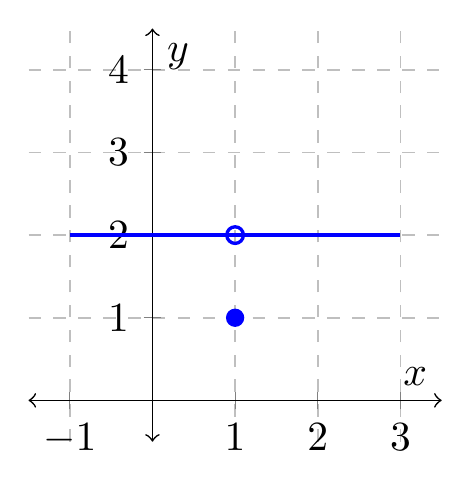
\begin{tikzpicture}[scale=1.5]
\begin{axis}[
    xlabel={$x$},
    xtick       = {-1,1,2,3,4},
    ytick       = {1,2,3,4},
    samples     = 160,
    domain      = -1:3,
    xmin = -1.5, xmax = 3.5,
    ymin = -0.5, ymax = 4.5,
    grid=both, grid style=dashed,
    width=2in, height=2in
]
% function approaching 2
\addplot[blue, thick] {2};
% open circle at (1,2)
\addplot[only marks, mark=o, blue, thick] coordinates {(1,2)};
% filled point at (1,1)
\addplot[only marks, mark=*, blue] coordinates {(1,1)};
\end{axis}
\end{tikzpicture}

\textcolor{blue}{
$\displaystyle \lim_{x\to 1} f(x) = 2$\\
$f(1) = 1$
}
\end{center}
\end{minipage}
%
\hfill
%
\begin{minipage}[t]{0.45\textwidth}
\begin{center}
\begin{tikzpicture}[scale=1.5]
\begin{axis}[
    xlabel={$x$},
    xtick       = {-1,1,2,3,4},
    ytick       = {1,2,3,4},
    samples     = 160,
    domain      = -1:3,
    xmin = -1.5, xmax = 3.5,
    ymin = -0.5, ymax = 4.5,
    grid=both, grid style=dashed,
    width=2in, height=2in
]
% left-hand side goes to +infinity
\addplot[
    blue,
    thick,
    domain=-1:0.98,
    samples=200
] {1/(1-x)^2};
% right-hand side constant
\addplot[only marks, mark=o, blue, thick] coordinates {(1,3)};

\addplot[blue, thick, domain=1:3] {3};
\end{axis}
\end{tikzpicture}

\textcolor{blue}{
$\displaystyle \lim_{x\to 1^-} f(x)$ DNE\\
$\displaystyle \lim_{x\to 1^+} f(x)$ exists
}
\end{center}
\end{minipage}

\begin{enumerate}
\item[(c)] For each of the two graphs you've sketched above, which continuity condition(s) are violated at $x=1$?

\textcolor{blue}{
\begin{itemize}
    \item \textbf{First graph:} Condition (iii) is violated.
    \item \textbf{Second graph:} Conditions (i),(ii) and (iii) are violated.
\end{itemize}
}
\end{enumerate}

%%%%%%%%%%%%%%%%%%%%%%%%%%%%%%%%%%%%%%%%%%%%%%%%%%%%%
%%%%%%%%%%% END PROBLEM L1 %%%%%%%%%%%%%%%%%%%%%%%%%%
%%%%%%%%%%%%%%%%%%%%%%%%%%%%%%%%%%%%%%%%%%%%%%%%%%%%%

\newpage

%%%%%%%%%%%%%%%%%%%%%%%%%%%%%%%%%%%%%%%%%%%%%%%%%%%%%
%%%%%%%%%%% BEGIN PROBLEM P1 %%%%%%%%%%%%%%%%%%%%%%%%
%%%%%%%%%%%%%%%%%%%%%%%%%%%%%%%%%%%%%%%%%%%%%%%%%%%%%

\item Each lottery ticket has a 1\% chance of paying out \$100 and a 10\% chance of paying out \$10. Otherwise the payout is \$0.

Let $X$ be a discrete random variable representing the amount a lottery ticket pays out.

\begin{enumerate}
    \item What are the possible values of $X$?

    \vspace{0.5cm}
    {\color{blue} $$S_X = \big\{ \$0,\ \$10,\ \$100\big\}$$} 
    \vspace{0.5cm}

    \item Write down the probability mass function $p(x)$ of $X$ using either a table or a piecewise function.

    \vspace{0.5cm}
    \begin{center}
        \color{blue}
 
        \begin{tabular}{c|ccc}
            \hline
           $x$  & 0 & 10 & 100 \\
           \hline
           $p(x)$  & 0.89 &  0.1 & 0.01\\
           \hline
        \end{tabular}
    \end{center}
    \vspace{0.5cm}

    \item Find the expectation of $X$.
    \vspace{0.5cm}
    {
    \color{blue}
        $$\mathbb{E}[X] = \sum_{x \in S_X} x\cdot p(x) = 0\cdot0.89+10\cdot 0.1+100\cdot0.01 = 2$$
    }
    \vspace{0.5cm}
    \item Find the variance of $X$.
    \vspace{0.5cm}
    {
    \color{blue}
        $$\mathrm{Var}[X] = \left(\sum_{x \in S_X} x^2\cdot p(x)\right) -\Big(\mathbb{E}[X]\Big)^2  = 0^2\cdot0.89+10^2\cdot 0.1+100^2\cdot0.01 -2^2 = 106$$
    }
    \vspace{0.5cm}



\end{enumerate}

%%%%%%%%%%%%%%%%%%%%%%%%%%%%%%%%%%%%%%%%%%%%%%%%%%%%%
%%%%%%%%%%% END PROBLEM P1 %%%%%%%%%%%%%%%%%%%%%%%%%%
%%%%%%%%%%%%%%%%%%%%%%%%%%%%%%%%%%%%%%%%%%%%%%%%%%%%%

\newpage

%%%%%%%%%%%%%%%%%%%%%%%%%%%%%%%%%%%%%%%%%%%%%%%%%%%%%
%%%%%%%%%%% BEGIN PROBLEM P2 %%%%%%%%%%%%%%%%%%%%%%%%
%%%%%%%%%%%%%%%%%%%%%%%%%%%%%%%%%%%%%%%%%%%%%%%%%%%%%

\item Let $X$ be a continuous random variable with the following probability density function.

\[p(x)=\begin{cases}cx^2\qquad -1\le x\le 2\\ 0 \qquad \text{otherwise}\end{cases}\]

\begin{enumerate}
    \item What is the support of $X$?

    {\color{blue}Solution: $[-1, 2]$, because this is the interval where $p(x) \neq 0$, as shown in the definition above.}

    \vfill

    \item Find the value of $c$ that makes $p(x)$ a valid probability density function.

    {\color{blue}Solution: We use the fact that $\int_{S_X} p(x) dx = 1$, where $S_X$ is the support of $X$. Using our previous answer, we obtain that

    $$1 = \int_{S_X} p(x) dx = \int_{-1}^2 cx^2 dx = c \int_{-1}^2 x^2 dx = c \frac{x^3}{3} \bigg|_{-1}^2 = c \left( \frac{2^3}{3} - \frac{(-1)^3}{3} \right) = c (3)$$
    
    Hence we obtain that $3c = 1$, so solving for $c$, we get that $c = \frac{1}{3}$.}

    \vfill
    
    \item Find the formula of the cumulative distribution function $C(x)$ of $X$ on the support of $X$.

    {\color{blue}From the previous problem, substituting $c = \frac{1}{3}$, we know that 

    \[p(x)=\begin{cases}\frac{x^2}{3}\qquad -1\le x\le 2\\ 0 \qquad \text{otherwise}\end{cases}\]
    
    Hence, we recall that $C(x) = \int_{-1}^x p(t) dt$, so we obtain that

    $$C(x) = \int_{-1}^x p(t) dt = \int_{-1}^x \frac{t^2}{3} dt = \frac{t^3}{9} \bigg|_{-1}^x = \frac{x^3}{9} - \frac{(-1)^3}{9} = \frac{x^3 + 1}{9}$$}

    \vfill

    \item Find $P(0<X<2)$.

    {\color{blue} We can use the probability density function:
    
    $$P(0<X<2) = \int_0^2 p(x) dx = \int_0^2 \frac{x^2}{3} dx = \frac{x^3}{9} \bigg|_0^2 = \frac{2^3}{9} - \frac{0^3}{9} = \frac{8}{9}$$
    
    OR we can use the cumulative density function:
    
    $$P(0<X<2) = C(2) - C(0) = \frac{2^3 + 1}{9} - \frac{0^3 + 1}{9} = \frac{9}{9} - \frac{1}{9} = \frac{8}{9}$$}

    \vfill
\end{enumerate}

%%%%%%%%%%%%%%%%%%%%%%%%%%%%%%%%%%%%%%%%%%%%%%%%%%%%%
%%%%%%%%%%% END PROBLEM P2 %%%%%%%%%%%%%%%%%%%%%%%%%%
%%%%%%%%%%%%%%%%%%%%%%%%%%%%%%%%%%%%%%%%%%%%%%%%%%%%%

\end{enumerate}

\end{document}